\documentclass[11pt]{article}

% \usepackage[utf8]{inputenc}
\usepackage{deauthor,times,graphicx}
\usepackage{hyperref}
\usepackage{algorithm}
\usepackage{algpseudocode}
\usepackage{amsmath}
\graphicspath{{figs/}}

\begin{document}

\title{College-Related Question Answering based on Knowledge Graph}
\author{Cheng Peng,  Hao Jiang, Junnan Dong, Xiao Huang\\
Department of Computing, The Hong Kong Polytechnic University
}

\maketitle

\begin{abstract}
An effective conversational agent can facilitate student advising. Many question-answering (QA) systems have been developed, but college-related QA has yet to be explored. It is a challenging task since questions from college students are domain-specific, while related training data is not available. The topics of the college-related questions are diverse, including the university, the department, undergraduate/graduate programs, and course content. To bridge this gap, we propose an effective question-answering framework for The Hong Kong Polytechnic University and Computer Science. It integrates a rule-based module, a knowledge-graph-based module, and a content-based module. The rule-based module can answer simple questions actually based on pre-defined rules. Then, we manually construct a college-related knowledge graph (KG) from related websites, Wikipedia, and textbooks. We embed the KG and employ the entity/relation representations to predict the answers. Moreover, we utilize a pre-trained language model to answer difficult questions based on college-related corpora. We evaluate the proposed QA framework by employing fourteen postgraduate students. The results show that it can answer most real-world questions.
\end{abstract}
%Question answering (QA) about college-related topics has been one of the major concerns of college education as the automatic pedagogical advice. Traditional QA systems leverage information retrieval techniques and natural language processing to provide answers to human-inputted questions. However, this is not applicable to specific domains, e.g., college-related questions. To bridge this gap, we propose a new QA system based on a domain knowledge graph (KG). Specifically, we manually extracted entities and relations from wikipedia and textbooks to construct the KG. We effectively learn the KG representation from its semantics and topology. The answers are predicated based on the obtained embedding in the form of a triple (head entity, predicate, tail entity). Moreover, we design two additional modules, i.e., rule-based and content-based components to strengthen the whole QA system for more complicated real-world questions with pre-defined rules and college-related corpus. The system is extensively tested by 14 postgraduate students. We comprehensively evaluate the model performance on the prediction of both the final questions and the detection of head/tail entities and relations from the inputted natural language questions.

\maketitle

\section{INTRODUCTION}
Knowledge Graphs (KGs) are an effective graph data structure modeling relational information. They consist of real-world entities and each entity's relations, corresponding to the nodes and edges in KG respectively \cite{c1, c2}. In KGs, each edge with its head entity and tail entity constitutes a triple (fact), i.e., (head entity, predicate, tail entity) or (h, p, t). To facilitate downstream tasks like Question Answering (QA) with abundant knowledge in KGs, Question Answering over Knowledge Graph (KGQA) is proposed \cite{c3, c4}. The main problem setting of KGQA is to translate the inputted natural language question into structured queries, and return the entities or predicates from KG as the answer. For example, given the question ``How tall is YAO Ming?'', the KGQA will translate this question to the query ``(YAO Ming, Height, ?)'', and return the answer by identifying this query's corresponding fact in KG ``(YAO Ming, Height, 2.29m)''.

This paper adopts a knowledge graph on special domains as the knowledge source for answers. Unlike other traditional KGQAs, which employ public large-scale KG databases including Freebase~\cite{Bollacker-etal08Freebase}, DBpedia \cite{c13}, and YAGO \cite{c14}, this paper mainly targets to provide QA service to college students, answering the questions related to Hong Kong Polytechnic University (PolyU) and Computer-Science (CS), while triple facts for these two college-related domains are not included in the existing public knowledge graphs. To construct the corresponding domain knowledge graph, we are required to collect domain information for the Hong Kong Polytechnic University and Computer-Science domains from Wikipedia, textbooks, and related websites.

However, some collected entities/predicates may have names different from those stored in KG, so translating natural language questions into KG queries needs to identify many different expressions in natural language questions \cite{c8, c9}. To solve this problem, we apply knowledge graph embedding \cite{c9, c11}, which can learn a vector representation for each entity and predicate in the knowledge graph. Similar entities or predicates will have similar vectors. Although this way is good at matching similar entities, when there are misspelled words on entities extracted from questions, the performance is affected significantly. Hence, to make the Knowledge Embedding based Knowledge Graph Question Answering (KEQA) more powerful, we also design an entity matching algorithm to help KEQA to correct those wrong words.

What's more, as the domains of inputted questions are always unbounded while any KG is far from completion \cite{c15}, for example, an unseen question's entity/predicate not involved in KG, it means that KGQA could not answer all the questions. To alleviate this problem, we add a content-based Question Answering (content-based QA) component to the whole QA framework, which consists of an advanced model standing for bidirectional encoder representations from transformers, just like the BERT \cite{c16}. By finetuning, the pre-trained model can search for answers from the collected text materials. Although we have extracted some triples from those materials, there is still much remaining knowledge. Adding them to the framework can expand the answerable range, but the processing speed of content-based QA is relatively slow, so it is only used as an alternative scheme. In addition, considering answering some simple questions immediately rather than using time-consuming machine learning models, the whole QA framework also includes a rule-based Question Answering (rule-based QA) component to improve the user experience and reduce the workload of the KGQA component.


In summary, rather than just relying on the advanced KGQA, the whole QA framework includes three different kinds of QA components. We design the rules for switching each QA component in our framework, which can make good use of every QA component. Eventually, we have a powerful QA framework in college-related domains. Our main contributions are presented as follows.
\begin{itemize}
  \item We deliver a QA framework for college-related questions, including three different kinds of QA components, which make the whole QA framework powerful.
  \item We define the rules to switch each QA component in the whole QA framework.
  \item A domain knowledge graph is constructed which covers the PolyU and Computer-Science domains.
  \item We achieve performance improvement of the traditional KGQA by adding knowledge graph embedding and entity matching algorithm.
\end{itemize}



\section{METHODOLOGY}
The whole QA framework in this paper has three components: rule-based Question Answering (rule-based QA), Question Answering over Knowledge Graph (KGQA), and content-based Question Answering (content-based QA).

\subsection{Overall Architecture of the Proposed Framework}
The whole QA framework is mainly relying on the KGQA. After constructing more than 15000 Hong Kong Polytechnic University (PolyU) and Computer-Science (CS) related triples, this huge PolyU and CS knowledge graph could cover most of the user's questions in these two domains. Especially with the improvement of knowledge graph embedding \cite{c9, c11} and entity matching algorithm, the KGQA component can deal with those questions with different expressions in entities or predicates.

However, KGQA still faces two challenges: (i) time-consuming for KG reasoning and (ii) knowledge-agnostic to those questions that KG does not cover.

As KGQA employs language models (three language models in this paper's KGQA component) to process questions, it is relatively time-consuming. For those questions with simple grammatical structure and the same expression of entity in the knowledge graph, there is no necessity to use KGQA models. For example, given the question ``Where is library?'', assuming that ``library'' is an entity as same as the ``library'' entity expression in the knowledge graph, it is empirically a question about locations, so the query in KG will be ``(Library, Location, ?)''. To answer these one-hop questions without using language models, the rule-based QA component is proposed. By matching manually-created regular expressions, the rule-based QA component could answer a lot of questions without using language models, which is much quicker than the KGQA component.

For those triples that the knowledge graph doesn't cover, KGQA could not answer the questions related to them. For instance, KGQA could not answer the question ``What's the use of loss function?'' if there is not a triple like ``(Loss Function, Use, xxx)'' in the knowledge graph. Though we collect many documents about PolyU and CS, there is still much knowledge that we do not extract from the textbooks. Introducing a content-based QA component could facilitate QA by making full use of text material in the database. After adding the content-based QA component, the QA framework could answer more questions than that only based on KG.

The overall architecture of our proposed QA system is illustrated in Figure 1. The rule-based QA component is added before the KGQA component. It will try to answer the question first without using time-consuming language models. The content-based QA component is added after the KGQA component, for answering those questions that KGQA is not able to answer but answerable in the textbook database.




The basic switching rules for each QA component are as follows. Initially, the inputted question will be delivered to the rule-based QA component to check whether there is any regular expression rule matched. If the question could not find the corresponding regular expression rule, it will be sent to the KGQA component. If KGQA could not answer the question (two cases: KGQA could not find the corresponding head entity in the knowledge graph; the distance between the predicted triple embedding representation and its nearest triple in candidates is larger than the pre-defined distance threshold), the question will be sent to content-based QA component. If the question could not be answered by content-based QA (the output score is lower than the pre-defined score threshold), it means that the whole QA framework is unable to answer this question.

\begin{figure}[t!]
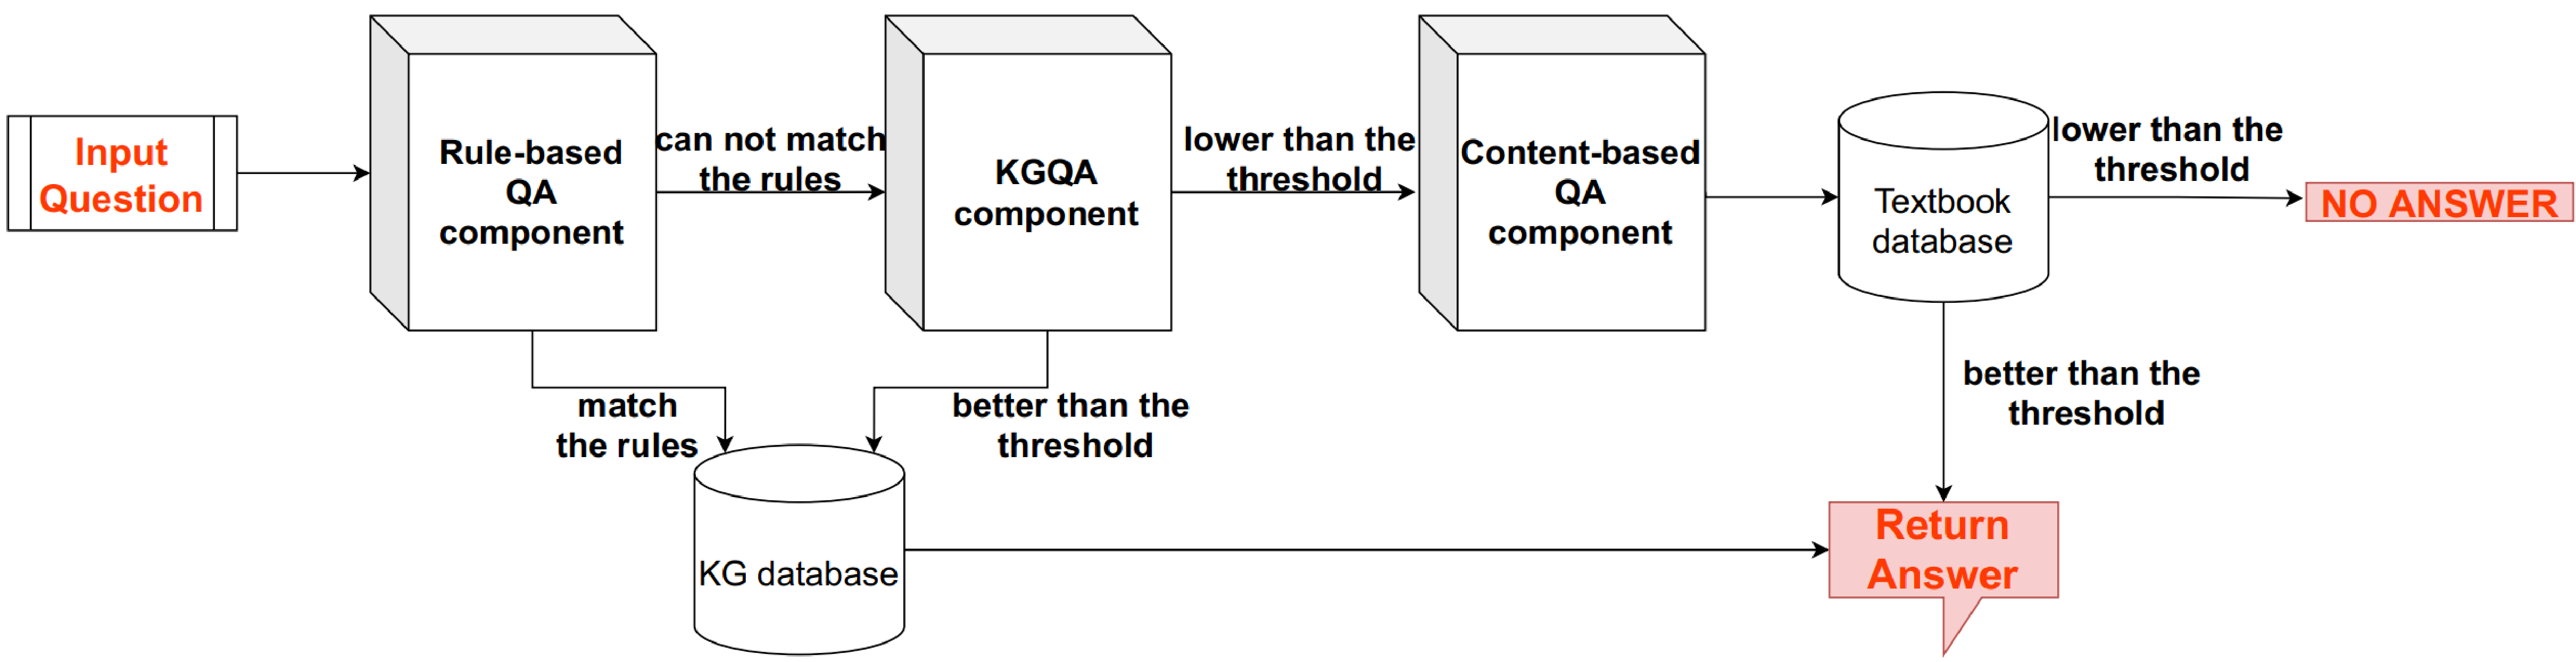
\includegraphics[width=17cm]{submissions/kbqa-colledge/figs/figure1.pdf}
\caption{The architecture of the proposed question answering framework.}
\end{figure}


\subsection{Construction of College-related Knowledge Graph }\label{sec:Knowledge Graph Construction}
The methods of constructing PolyU and CS related knowledge graphs in this paper are shown as follows. (i) Manually browsing or using python crawler technology to collect knowledge on the official websites, such as Hong Kong Polytechnic University (PolyU) main page. After equipping with the knowledge, we transform the knowledge into triples like ``(VA Student Canteen, Location, G/F, Shaw Amenities Building (Core VA))''. (ii) Using Wikipedia (a Python library)\footnote{\url{https://pypi.org/project/wikipedia/}} to access and parse data from Wikipedia. Similar to the first method, we transform the knowledge to a triple format \cite{c1, c2}. (iii) Manually collecting some textbooks and using a pre-trained reading comprehension model \cite{c19} to search the corresponding tail entity that we want. For example, we use the reading comprehension model to search for the answer of ``Who is the inventor of JAVA?'' from JAVA textbook. If the returned text is ``James Gosling'', which is a correct answer, we will transform it to a triple ``(JAVA, inventor, James Gosling)''.

Based on the above three methods, there are more than $15$,$000$ PolyU and CS related triples constructed in total, which can answer a huge range of Hong Kong Polytechnic University and Computer-Science questions.






\subsection{Rule-based Question Answering}\label{sec:RULE-BASED QA}
The first question answering component in this paper is the rule-based Question Answering (rule-based QA) component. This kind of approach is one of the initial methods used by traditional QA systems \cite{c30}, which uses different kinds of rules, e.g., semantic rules and keywords, to understand the intentions of inputted questions. Furthermore, it is also used to assist other types of QAs, especially KGQA. For example, Z. Jiang et al. built a medical lexicon to classify and query questions in KGQA through rule-based matching methods and string-matching algorithms \cite{c31}.

Similarly, the rule-based QA component in our paper extracts entities and predicates from questions based on the string matching algorithms. By matching the questions with pre-defined regular expressions, we could get the head entities and predicates in questions without using any time-consuming models.

However, due to the limitations of labor-consuming rule mining, we merely use the rule-based component to process two types of questions. The first one is simple and common questions, such as ``Where is library?'', which is used for increasing the whole QA framework processing speed. When the component receives a question, it will initially check whether the question contains pre-defined question words in the rule dictionary for the first classification which aims to recognize the general intention. In the example above, the question will trigger the ``Where'' rule for locations. Then, according to the recognized intention, the question will be allocated to the special rule dictionary for the second classification in which we design many keywords for regex matching. If the question matches any regular expression, the corresponding predicate will be determined. Consequently, all the entities related to the predicate in our database will be identified. Finally, based on Levenshtein Distance, we calculate the distance between the head entity candidates and the text except for pre-defined rule keywords in question. The closest head entity candidate will be regarded as the final head entity result. The tail entity obtained by the head entity and predicate in the knowledge database is the final answer to the question. The second type is questions that need some simple operations after detecting predicates and head entities rather than just returning the tail entity as the answer, such as the summation in ``How many elective courses in MSc. IT?''. Under such circumstances, the predicate and head entity detection is the same as that for the first type. The only difference is that processing the second question type requires additional operation after head entity and predicate recognition. For different operations, we formulate different rules in the rule-based QA component, such as counting the number of tail entities. For the example question, after recognizing ``Elective Courses'' as the predicate and ``IT MSc'' as the head entity, calculating the number of tail entities in the triple pattern ``(IT MSc, Elective Courses, ?)'' is necessary for obtaining the final answer. Therefore, we set the rule that after recognizing the intention of ``Number'' and the predicate of ``Elective Courses'', the rule-based QA component needs to calculate the number of elective courses.





\subsection{Question Answering based on Knowledge Graph Embedding}\label{sec:Knowledge Embedding Based KGQA}
In our framework, in order to better identify the head entity and predicate by recognizing different expressions of entity/predicate in natural language questions \cite{c8,c9} correctly, the knowledge graph embedding \cite{c9, c11} is applied to the KGQA component, which can learn a vector representation for each predicate and entity in knowledge graph and keep the original relations simultaneously. What's more, because there is a large number of triples in the knowledge graph, it's very expensive and noisy to compare the predicted triple with all the triples in KG database. Therefore, we introduce a head entity detection model which could effectively prioritize the candidate triples. For example, given the question ``Where is VA canteen?'', the detected head entity is ``VA canteen''. The candidate triples to be compared will only be the ones with the head entity ``VA canteen''. The main idea of the KGQA component based on knowledge graph embedding in this paper is illustrated in Figure 2.

\begin{figure}[htp]
    \centering
    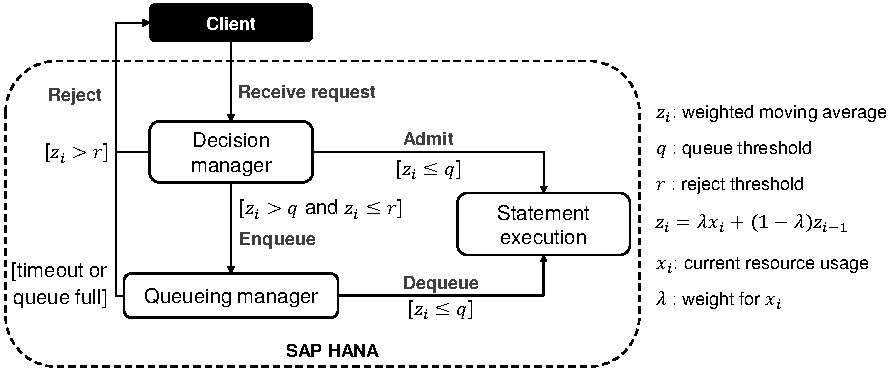
\includegraphics[width=17cm]{submissions/kbqa-colledge/figs/figure2.pdf}
    \caption{The workflow of the KGQA component.}
\end{figure}




\begin{table}[h!]
\footnotesize
\caption{The notations in KGQA component and corresponding definitions.}
\centering
\begin{tabular}{c c}
 \hline
 Notations & Definitions  \\ [0.2ex]
 \hline
 G & this framework's knowledge graph  \\
 Q & the questions in training set  \\
 (h, p, t) & a triple (fact) in G, (head entity, predicate, tail entity)  \\
 d & dimension of entity/predicate embedding representation  \\
 ${\mathbf{e}}_h$ $\in$ $ \mathbf{R}^{1*d}$ & head entity embedding representation vector  \\
 ${\mathbf{e}}_p$ $\in$ $ \mathbf{R}^{1*d}$ & predicate embedding representation vector  \\
 ${\mathbf{e}}_t$ $\in$ $ \mathbf{R}^{1*d}$ & tail entity embedding representation vector  \\
 $\hat{\mathbf{e}}_h$ $\in$ $ \mathbf{R}^{1*d}$ & predicted head entity embedding representation vector  \\
 $\hat{\mathbf{e}}_p$ $\in$ $ \mathbf{R}^{1*d}$ & predicted predicate embedding representation vector  \\
 $\hat{\mathbf{e}}_t$ $\in$ $ \mathbf{R}^{1*d}$ & predicted tail entity embedding representation vector  \\
 HED & Head Entity Detection model  \\
 ${\mathbf{HED}}_{entity}$ & detected head entity token in HED  \\
 ${\mathbf{HED}}_{non}$ & detected non head entity token in HED  \\
 \hline
\end{tabular}
\label{table:KGQA}
\end{table}

To better describe the workflow of KGQA, we summarize the significant notations in Table~\ref{table:KGQA}.
The question answering process of the KGQA component is mainly five steps: (i) Input the question into the Head Entity Detection (HED) model to get ${\mathbf{HED}}_{entity}$ and  ${\mathbf{HED}}_{non}$. (ii) Generate the candidate-triple set from the KG database by the detected head entity name ${\mathbf{HED}}_{entity}$. (iii) Input the question into the predicate representation model to get $\hat{\mathbf{e}}_{p}$. (iv) Input the question into the head entity representation model to get $\hat{\mathbf{e}}_{h}$. (v) For all triples in the candidate triple set, calculate each one's distance to the predicted triple ($\hat{\mathbf{e}}_{h}$, $\hat{\mathbf{e}}_{p}$, $\hat{\mathbf{e}}_{t}$), and return the nearest candidate triple as the answer.

There are two cases in which the KGQA component is not able to answer the questions. Firstly, in the above (ii) step, KGQA may not find the corresponding head entity in the knowledge graph. Secondly, in the above (v) step, the distance between the predicted triple ($\hat{\mathbf{e}}_{h}$, $\hat{\mathbf{e}}_{p}$, $\hat{\mathbf{e}}_{t}$) and its nearest triple in candidates may be larger than the pre-defined distance threshold. If one of the above cases happens, the question will be sent to the content-based QA component.



\subsubsection{Head Entity Detection Model}\label{sec:Head Entity Detection Model}
In the first step of the KGQA component, there is a Head Entity Detection (HED) model which aims to find target tokens (words) in the question for the head entity, so that the candidate triples will be the triples with the same or similar detected head entity names, rather than all triples in KG. The predicted representation of head entity $\hat{\mathbf{e}}_h$ from the representation model is used for dealing with ambiguity.

We adopt the long short-term memory (LSTM) \cite{c20} structure, which is a bidirectional recurrent neural network to facilitate a concise KGQA module. Figure 3(a) shows the architecture of HED model.


Given a question with length L, the HED model will use a pre-trained model (GloVe \cite{c21}) to map it to an L-length sequence of word embedding vectors $\mathbf{x}_j$ (for j = 1, …, L). Then, there is the bidirectional LSTM \cite{c20} structure to generate $\mathbf{h}_j$. After the LSTM structure, a fully connected layer and a softmax function are applied to $\mathbf{h}_j$, generating the final vector $\mathbf{v}_j$ $\in$ $\mathbf{R}^{(2*1)}$ for each token in this L-length sentence. The two values in $\mathbf{v}_j$ represent the probabilities that the $\mathbf{j}^{th}$ token belongs to the entity name token and non-entity name token respectively. If the probability of the entity name token is higher, it will be classified as ${\mathbf{HED}}_{entity}$. To sum up, HED model can classify each token in question whether it is a token in the head entity, and finally connect one or several tokens as the head entity name. We denote these tokens as ${\mathbf{HED}}_{entity}$, and the remaining tokens in question as ${\mathbf{HED}}_{non}$.

To train the Head Entity Detection (HED) model, this paper uses the questions in training set Q as training data input and tags their head entity names as the training data output. For instance, the training question ``Where is VA canteen'' is tagged as ``O O I I'' in which ``O'' stands for ${\mathbf{HED}}_{non}$, and ``I'' means ${\mathbf{HED}}_{entity}$. After training, the HED model can identify which tokens in question are ${\mathbf{HED}}_{entity}$.


\begin{figure}[htp]
    \centering
    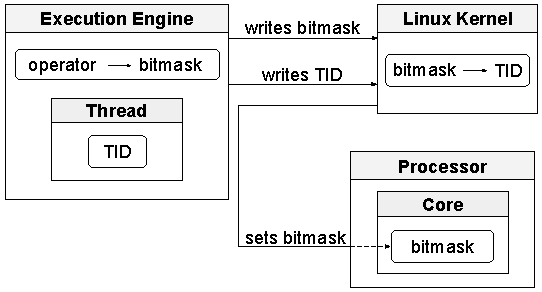
\includegraphics[width=15cm]{submissions/kbqa-colledge/figs/figure3.pdf}
    \caption{Architectures of head entity detection model and predicate/head entity representation model.}
\end{figure}


\subsubsection{Knowledge Graph Embedding}\label{sec:Knowledge Graph Embedding}
Knowledge graph embedding \cite{c9, c11} could represent each predicate and entity in the knowledge graph as a vector, while the triple's original structure and relation in the knowledge graph are well-preserved in those embedding vectors. The reason why this paper uses knowledge embedding is that it can disambiguate those inputted questions' head entity name or predicate name which is different from the corresponding entity name or predicate name in the knowledge graph database. The traditional KGQA is hard to deal with this issue while Knowledge Embedding based Knowledge Graph Question Answering (KEQA) could potentially improve the question answering accuracy in this case.

There are many different kinds of knowledge graph embedding algorithms \cite{c9, c11}, and the basic ideas of most knowledge graph embedding algorithms \cite{c15, c22, c23} are similar. For each triple (h, p, t) in knowledge graph G, denoting its knowledge graph embedding representation as ($\mathbf{e}_h$, $\mathbf{e}_p$, $\mathbf{e}_t$), which are three vectors for h, p, t respectively. The knowledge graph embedding algorithm will initialize  $\mathbf{e}_h$, \ $\mathbf{e}_p$ and $\mathbf{e}_t$ randomly \cite{c15, c22} (or use word embedding model to initialize \cite{c24, c25}). In addition, each knowledge graph embedding algorithm has a unique function f (·), which could represent the tail entity vector by head entity vector and predicate vector in the same triple ($\mathbf{e}_t$ $\approx$ f ($\mathbf{e}_h$, $\mathbf{e}_p$)). Finally, the embedding algorithm's target is to minimize the distance between $\mathbf{e}_t$ and f ($\mathbf{e}_h$, $\mathbf{e}_p$) for all the triples in the knowledge graph G by training, while the training step is using both positive and negative samples in KG. Each knowledge graph embedding algorithm is mainly different in the function f (·).

In this paper, TransE \cite{c22}, a typical knowledge graph embedding method is picked, which defines the ``$\mathbf{e}_t \approx \mathbf{e}_h + \mathbf{e}_p$'' relation (function f (·)) for each triple ($\mathbf{e}_h$, $\mathbf{e}_p$, $\mathbf{e}_t$) in KG. We apply TransE to initialize the values of $\mathbf{e}_h$, $\mathbf{e}_p$ and $\mathbf{e}_t$ randomly at the first stage, and then minimize the overall distance between $\mathbf{e}_t$ and f ($\mathbf{e}_h$, $\mathbf{e}_p$) by training. After training, we obtain the embedding vectors of the head entity and predicate in one specific triple, which are $\mathbf{e}_h$ and $\mathbf{e}_p$; then, we can calculate the representation vector of the tail entity ($\mathbf{e}_t$) in this triple automatically, which is $\mathbf{e}_h + \mathbf{e}_p$.


\subsubsection{Predicate and Head Entity Representation Models}\label{sec:Predicate and Head Entity Representation Models}
The target of predicate and head entity representation models is outputting the predicate representation vector $\hat{\mathbf{e}}_p$ and head entity representation vector $\hat{\mathbf{e}}_h$ in the knowledge graph embedding space by the given question. The input of the representation model is a natural language question, and the output is a vector.

For the representation model, to keep neural network architecture simple, similar to the previous HED model, the representation model mainly consists of a bidirectional long short-term memory (LSTM) structure \cite{c20}. The part difference with the HED model is that the representation model's output (head entity/predicate representation vector) is related to every token in question, so an attention layer is added, which could take the order and the importance of all words into consideration.

The predicate and head entity representation models' architecture is shown in Figure 3(b). The workflow before the attention layer (given a question with length L) is similar to that of the HED model. After the attention layer and concatenation, each token will generate a vector $\mathbf{r}_j$ (for j = 1, …, L). Finally, the predicted predicate/head entity representation vector is computed by the mean of all $\mathbf{r}_j$, which is $\hat{\mathbf{e}}_{p}/\hat{\mathbf{e}}_{h}=\frac{1}{L} \sum_{j=1}^L \mathbf{r}_j^{\top}$ .

To train the predicate and head entity representation models, we need to label each question's corresponding predicate/head entity representation vector ${\mathbf{e}}_p$/$\mathbf{e}_h$. After training, the predicted output vector $\hat{\mathbf{e}}_p$/$\hat{\mathbf{e}}_h$ of inputted question will be close to this question's real predicate/head entity knowledge graph embedding representation vector ${\mathbf{e}}_p$/$\mathbf{e}_h$.





\subsubsection{Joint Search on Embedding Spaces}\label{sec:Joint Search on Embedding Spaces}
After obtaining the candidate triples from the HED model as well as predicted predicate representation $\hat{\mathbf{e}}_p$ and predicted head entity representation $\hat{\mathbf{e}}_h$ from corresponding representation models, the next step of the KGQA component is to find the triple from all the candidates which best matches the predicted $\hat{\mathbf{e}}_p$ and $\hat{\mathbf{e}}_h$.

Let C be the set of candidate triples generated from the HED model. In order to calculate the distance between each candidate triple (h, p, t) and the predicted triple representation vector ($\hat{\mathbf{e}}_h$, $\hat{\mathbf{e}}_p$, $\hat{\mathbf{e}}_t$), this framework makes full use of the relation ${\mathbf{e}}_t$ $\approx$ f (${\mathbf{e}}_h$, ${\mathbf{e}}_p$) = (${\mathbf{e}}_h$ + ${\mathbf{e}}_p$) in TransE \cite{c22}, which means that the predicted tail entity representation $\hat{\mathbf{e}}_t$ could be computed by predicted predicate representation $\hat{\mathbf{e}}_p$ and predicted head entity representation $\hat{\mathbf{e}}_h$. Thus, a direct way to compute the distance between the predicted triple vector and each triple embedding representation vector (${\mathbf{e}}_h$, ${\mathbf{e}}_p$, ${\mathbf{e}}_t$) in candidate triples is achieved by the sum distance of $\hat{\mathbf{e}}_h$ and ${\mathbf{e}}_h$, $\hat{\mathbf{e}}_p$ and ${\mathbf{e}}_p$, $\hat{\mathbf{e}}_t$ and ${\mathbf{e}}_t$. Moreover, as the real final-selected head entity name in C is likely to be the same as ${\mathbf{HED}}_{entity}$, and the predicate name is also likely to be mentioned in the other text of the question (${\mathbf{HED}}_{non}$) \cite{c26}, the joint distance metric is proposed as follows.
\begin{equation}
    \underset{(h, p, t) \in C}{\operatorname{minimize}} \left\|\mathbf{e}_{p}-\hat{\mathbf{e}}_{p}\right\|_2+\beta_1\left\|\mathbf{e}_h-\hat{\mathbf{e}}_h\right\|_2+\beta_2\left\|\mathbf{e}_t-(\hat{\mathbf{e}}_{h} + \hat{\mathbf{e}}_{p}\right)\|_2 -\beta_3 \operatorname{sim}\left[h, \mathbf{HED}_{\text {entity}}\right]-\beta_4 \operatorname{sim}\left[p, \mathbf{HED}_{\text {non}}\right].
    \label{eq:prediction}
\end{equation}


The first three terms are to calculate the distance between one candidate triple (h, p, t) and the predicted triple representation vector ($\hat{\mathbf{e}}_{h}$, $\hat{\mathbf{e}}_p$, $\hat{\mathbf{e}}_{t}$) while using ${\mathbf{l}}^2$ norm to measure the distance in embedding space. The final two terms are to check whether the head entity name (h) and predicate name (p) in candidate triple are mentioned in the question. Function sim() is used to calculate the string similarity. $\beta1$, $\beta2$, $\beta3$, and $\beta4$ are pre-defined weights \cite{c26}.





\subsubsection{Entity Detection Improvement}\label{sec:Entity Detection Improvement}
According to the workflow of the KGQA component, it's clear that generating the candidate triples by the detected head entity is important. After inputting the question into the head entity detection (HED) model, the HED model will judge which tokens in question constitute the head entity. However, there are three possible problems in this part, including the detected head entity containing some other tokens besides the correct head entity name, the detected head entity only being a part of the correct head entity name, and the detected head entity having some misspelled words. Any of these situations could cause entity matching to fail. If the detected head entity could not match any head entity in the knowledge graph, there will be no candidate triples. Correspondingly, the joint search in embedding spaces cannot play its role. Therefore, it is necessary to deal with the above three cases by entity detection improvement based on some string-matching algorithms.

For the first case, the detected head entity may include some unrelated tokens besides the original head entity name. For example, the detected head entity is ``the department of computing in PolyU'' while the head entity name stored in KG is ``department of computing''. In this case, we use N-Gram \cite{c27} algorithm to extract 1-gram, 2-gram to n-gram from each fragment in detected entity words, which will form a set of n-gram. Then, the framework will use the n-gram set to find head entities in the KG dataset, generating a set of detected head entity candidates. The remaining issues are detected head entity that is merely a part of the head entity name in KG or includes misspelled words. For instance, the correct head entity name in KG is ``department of computing'', while the detected head entity is ``computing department'' (a part of the correct head entity) or ``depart of computing'' (misspelled words). In the circumstances, the KGQA component is difficult to accurately generate the candidate triples from these two kinds of detected head entities. To match these two kinds of ``wrong-input'' head entity names in question, a string-matching algorithm named Monge and Elkan (Mon-Elk) based on Levenshtein \cite{c28} is added. It is a hybrid string-matching algorithm at character and token levels, which will calculate the similarity between each token in different sentences. The formula is shown in Eq.~\eqref{equ:match}. A and B are the strings that we want to calculate how similar they are, and $A_i$, $B_j$ are the tokens in A and B respectively.

\begin{equation}
    \operatorname{match}(A, B)=\frac{1}{|A|} \sum_{i=1}^{|A|} \max _{j=1}^{|B|} \operatorname{match}\left(A_i, B_j\right).
    \label{equ:match}
\end{equation}

Following prevailing studies \cite{c29}, n-gram combined with set-matching methods is the best matching algorithm for the matching problem. However, the experiment is done on data with no typing errors. Compared with the best method, the second best one, Mon-Elk based on Levenshtein, is more suitable for our applications, because Levenshtein edit distance can better determine the extent of spelling errors. After calculating the Mon-Elk similarity between the detected head entity and each entity in KG, the knowledge embedding based KGQA component will select those entities with a similarity larger than the pre-defined similarity threshold as head entity candidates and use them to generate the candidate triples.

\subsection{Content-based Question Answering}\label{sec:CONTENT-BASED QA}
The final component of our framework is content-based question answering (content-based QA). All the documents in this part are crawled by us from textbooks or through Wikipedia API. If this component is not able to provide the answer, the whole QA framework will return ``no answer'' as the final reply to users. In this part, we divide the content-based question answering component into two aspects, document retrieval and content reader. The general workflow of content-based QA is illustrated in Figure 4. In this paper, we deploy the content-based question answering component through an open end-to-end framework, haystack\footnote{\url{https://github.com/deepset-ai/haystack}}.


\begin{figure}[htp]
    \centering
    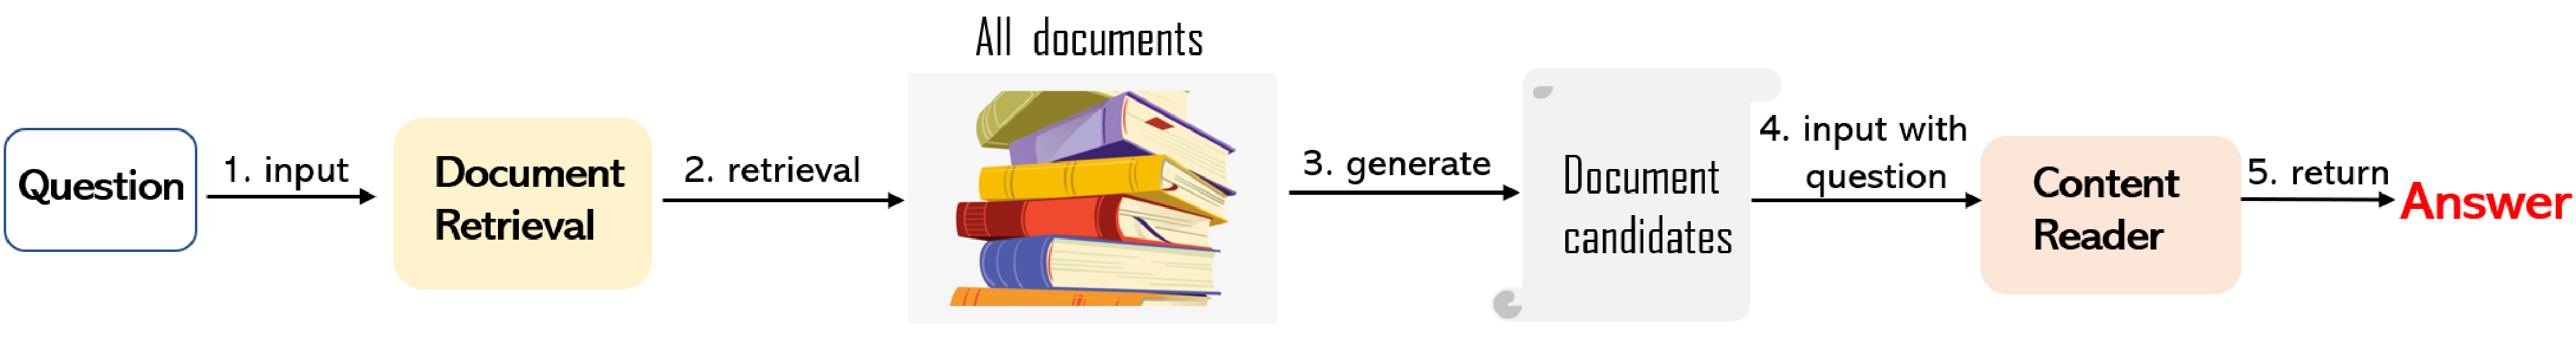
\includegraphics[width=17cm]{submissions/kbqa-colledge/figs/figure4.pdf}
    \caption{The workflow of content-based question answering component.}
\end{figure}


\subsubsection{Document Retrieval}\label{sec:CONTENT-BASED QA 1}
Generally, dense retrievers perform better than sparse methods, like TF-IDF and BM25, but dense approaches are computationally more expensive, especially during indexing \cite{c36}. Therefore, to make our framework more simplified and low computational complexity, we only perform the retrieval through a simple method, Term Frequency-Inverse Document Frequency (TF-IDF) which is a commonly used baseline for information retrieval. There are two main ideas of TF-IDF. Firstly, the more words the two documents overlap, the more relevant they are. In addition, the fewer documents a word is contained in, the more important the word is.

When the component receives a question, all the documents will be calculated TF-IDF score with it and sorted from largest to smallest according to the score. The top n documents will be prioritized as document candidates in which the content reader searches for answers. In our framework, we value the top two as the document candidates.

\subsubsection{Content Reader}\label{sec:CONTENT-BASED QA 1}
After retrieving the documents, the content reader takes a question and a set of candidate documents as inputs and returns an answer by selecting a text span within the documents. For selecting the reader model in this part, we choose an easy-to-deploy and powerful model -- RoBERTa \cite{c33}.


As it is expensive to manually annotate the span of documents and valid texts to train the content reader, we apply the pre-trained RoBERTa model by Deepset\footnote{\url{https://huggingface.co/deepset/roberta-base-squad2/}} on SQuAD2.0 dataset which includes both answerable and unanswerable questions. Compared with the model trained on SQuAD1.0/1.1 dataset, there is an additional binary classifier to automatically identify whether a question can be answered or not. The span predictor and classifier are trained jointly \cite{c33}. To fine-tune the model for our tasks, we create some question-answer pairs in our documents.


In terms of the process of the content-based QA component, the model takes a question and a set of candidate documents obtained by the document retrieval as input, returning a set of answers with a predicted score and no-answer score of the query. In our framework, we set 0 as the threshold of the no-answer score. If the no-answer score is higher than or equal to 0, it means that the question can be answered. In this case, the content-based QA component will return the result with the highest predicted score as the final answer. On the contrary, if the no-answer score is lower than the threshold, the question will be considered unanswerable. Since the content-based question answering module is the final part of our framework, when the query is considered unanswerable, the QA framework will return a no-answer signal to users directly.




\section{EXPERIMENTS}

After implementing the whole QA framework which includes three different QA components mentioned above, we design a website and embed the QA service interface for front-end users. After the users log in, they could talk with the chatbot for answers.

To evaluate the effectiveness of this proposed QA framework, we invite 14 students in the department of computing at PolyU and collect a total of 730 questions related to PolyU or Computer-Science. Since we regulate those testers to ask questions about PolyU and Computer-Science but do not limit the candidate concepts (entity names) and relations they could ask, there are some unbounded questions that our QA framework is not able to answer (no corresponding knowledge graph or text material in the database). Among all the 730 inputted questions, there are 638 valid questions. The term ``valid'' means that the knowledge graph database or text corpus in this paper is enough to deal with this specific question. So, for all these 14 students, our QA framework is possible to answer 87.4\% of all testers' questions. It means that this framework's database is capable to satisfy most general college students' needs.


\begin{table}[h!]
\caption{The accuracy of our question answering framework.}
\begin{center}
\begin{tabular}{ |c|c| }
  \hline
   & QA Framework Accuracy \\
  \hline
  PolyU domain & 87.1\% \\
  \hline
  CS domain & 80.6\% \\
  \hline
  PolyU \& CS domain & 83.6\% \\
  \hline
\end{tabular}
\end{center}
\end{table}


Table 2 shows the accuracy of the whole QA framework in this paper. For all those 638 valid questions, the QA framework could correctly answer 534 questions, which is up to 83.6\%. In addition, we also calculate the accuracies in PolyU and Computer-Science domains respectively: For questions related to Computer-Science domain, the accuracy is lower than the PolyU domain, which is mainly because the Computer-Science domain questions are more complex and multifaceted. They are more suitable to be processed by content-based QA component. For PolyU related questions, the KGQA component is sufficient to answer most of them, and we achieve relatively satisfying performance.

Although our proposed framework obtains good accuracy for answering college-related questions, there are still a lot of unbounded questions (12.6\%). In other words, if we include all the unbounded questions, the overall accuracy is 73.1\% (calculated by Eq.~\eqref{equ:overall}, $N_{valid}$ means the number of all valid questions in testing questions and $N_{all}$ means the number of all testing questions), which is far from perfect.

\begin{equation}
    Overall \ Accuracy= \frac{N_{valid}}{N_{all}} \ * \ {QA \ Framework \ Accuracy} .
    \label{equ:overall}
\end{equation}

To keep improving the overall accuracy, the direct way is constructing more knowledge graphs or collecting more text materials to make this framework more powerful.






\section{CONCLUSIONS AND FUTURE WORK}
In this paper, our target is to design a QA framework that can answer the questions related to Hong Kong Polytechnic University (PolyU) and Computer-Science (CS). Inspired by the KGQA that allows users access knowledge in some public knowledge graph databases, we construct the PolyU and CS related knowledge graph with more than 15000 triples to facilitate knowledge reasoning. In order to handle the ambiguity of different expressions, misspelled words, and partial names in questions, this paper improves the KGQA component by using knowledge graph embedding and off-the-shelf string-matching algorithms like the Mon-Elk matching algorithm and N-Gram. The KGQA component in this paper could have a better performance than the traditional simple KGQA.

In addition to KGQA, a rule-based QA component and content-based QA component are proposed to enhance the whole framework. Rule-based QA could answer some simple questions based on logical rules, while content-based QA is able to answer some unbounded questions that the knowledge graph doesn't cover but can be answered from rich texts.

After defining the rules for switching each QA component in the whole framework, we could make full use of each QA component and propose a powerful QA framework for answering college-related questions.

In future work, except for constructing more knowledge graphs and collecting more text materials, we will try to keep improving this QA framework through the following aspects. (i) We will apply more cutting-edge multi-hop knowledge graph reasoning algorithms for complex question answering. (ii) The continual learning ability for a conversational chatbot will be one of our main focuses to improve the usability of the framework.





\begin{thebibliography}{10}
\itemsep=1pt
\begin{small}


\bibitem{c1} Yankai Lin, Zhiyuan Liu, Maosong Sun, Yang Liu, and Xuan Zhu. \newblock  Learning Entity and Relation Embeddings for Knowledge Graph Completion. \newblock In {\em AAAI Conference on Artificial Intelligence}, 2181--2187, 2016.

\bibitem{c2} Quan Wang, Zhendong Mao, Bin Wang, and Li Guo. \newblock  Knowledge Graph Embedding: A Survey of Approaches and Applications. \newblock {\em IEEE Transactions on Knowledge and Data Engineering}, 29, 12:2724--2743, 2017.

\bibitem{c3} Zihang Dai, Lei Li, and Wei Xu.  \newblock  CFO: Conditional Focused Neural Question Answering with Large-Scale Knowledge Bases. \newblock In {\em Annual Meeting of the Association for Computational Linguistics}, 800--810, 2016.

\bibitem{c4} Yanchao Hao, Yuanzhe Zhang, Kang Liu, Shizhu He, Zhanyi Liu, Hua Wu, and Jun Zhao. \newblock  An End-to-End Model for Question Answering over Knowledge Base with Cross-Attention Combining Global Knowledge. \newblock {\em Annual Meeting of the Association for Computational Linguistics}, 221--231, 2017.

\bibitem{Bollacker-etal08Freebase}
Kurt Bollacker, Colin Evans, Praveen Paritosh, Tim Sturge, and Jamie Taylor.
\newblock Freebase: a collaboratively created graph database for structuring
  human knowledge.
\newblock In {\em International Conference on Management of Data}, pages
  1247--1250, 2008.

% \bibitem{c5} Scott Wen-tau Yih, Ming-Wei Chang, Xiaodong He, and Jianfeng Gao. \newblock  Semantic Parsing via Staged Query Graph Generation: Question Answering with Knowledge Base. \newblock {\em ACL-IJCNLP}, 2015.

% \bibitem{c6} Roi Blanco, Giuseppe Ottaviano, and Edgar Meij. \newblock  Fast and Space-Efficient Entity Linking for Queries. \newblock {\em WSDM}, 179–188, 2015.

% \bibitem{c7} Aasish Pappu, Roi Blanco, Yashar Mehdad, Amanda Stent, and Kapil Thadani.  \newblock  Lightweight Multilingual Entity Extraction and Linking. \newblock {\em WSDM}, 365–374, 2017.

\bibitem{c8} Jonathan Berant, Andrew Chou, Roy Frostig, and Percy Liang.  \newblock  Semantic Parsing on Freebase from Question-Answer Pairs. \newblock In {\em Conference on Empirical Methods in Natural Language Processing}, 1533--1544, 2013.

\bibitem{c9} Scott Wen-tau Yih, Ming-Wei Chang, Xiaodong He, and Jianfeng Gao.  \newblock Semantic Parsing via Staged Query Graph Generation: Question Answering with Knowledge Base. \newblock In {\em ACL-IJCNLP}, 1321--1331, 2015.

\bibitem{c11} Zhen Wang, Jianwen Zhang, Jianlin Feng, and Zheng Chen.  \newblock  Knowledge Graph and Text Jointly Embedding. \newblock In {\em Conference on Empirical Methods in Natural Language Processing}, 1591--1601, 2014.


\bibitem{c13} Jens Lehmann, Robert Isele, Max Jakob, Anja Jentzsch, Dimitris Kontokostas, Pablo N Mendes, Sebastian Hellmann, Mohamed Morsey, Patrick Van Kleef, Sören Auer, et al.  \newblock   DBpedia–A Large-Scale, Multilingual Knowledge Base Extracted From Wikipedia. \newblock {\em Semantic Web 6}, 2, 167--195, 2015.

\bibitem{c14} Fabian M Suchanek, Gjergji Kasneci, and Gerhard Weikum.  \newblock   YAGO: A Core of Semantic Knowledge. \newblock In {\em International World Wide Web Conference}, 697--706, 2007.

\bibitem{c15} Yankai Lin, Zhiyuan Liu, Maosong Sun, Yang Liu, and Xuan Zhu.  \newblock  Learning Entity and Relation Embeddings for Knowledge Graph Completion. \newblock In {\em AAAI Conference on Artificial Intelligence}, 2181--2187, 2015.

\bibitem{c16} Jacob Devlin, Ming-Wei Chang, Kenton Lee and Kristina Toutanova. \newblock BERT: Pre-training of Deep Bidirectional Transformers for Language Understanding. \newblock In {\em NAACL-HLT}, 4171--4186, 2019.


\bibitem{c19} Pranav Rajpurkar, Jian Zhang, Konstantin Lopyrev, Percy Liang.  \newblock   SQuAD: 100,000+ Questions for Machine Comprehension of Text. \newblock In {\em Conference on Empirical Methods in Natural Language Processing}, 2016.

\bibitem{c20} Dzmitry Bahdanau, Kyunghyun Cho, and Yoshua Bengio.  \newblock  Neural Machine Translation by Jointly Learning to Align and Translate. \newblock In {\em International Conference on Learning Representations}, 2015.

\bibitem{c21} Jeffrey Pennington, Richard Socher, and Christopher Manning. \newblock  GloVe: Global Vectors for Word Representation. \newblock In {\em Conference on Empirical Methods in Natural Language Processing}, 1532--1543, 2014.

\bibitem{c22} Antoine Bordes, Nicolas Usunier, Alberto Garcia-Duran, Jason Weston, and Oksana Yakhnenko. \newblock  Translating Embeddings for Modeling Multi-relational Data. \newblock In {\em Annual Conference on Neural Information Processing Systems}, 2787--2795, 2013.

\bibitem{c23} Han Xiao, Minlie Huang, Lian Meng, and Xiaoyan Zhu. \newblock  SSP: Semantic Space Projection for Knowledge Graph Embedding with Text Descriptions. \newblock In {\em AAAI Conference on Artificial Intelligence}, 3104--3110, 2017.

\bibitem{c24} Teng Long, Ryan Lowe, Jackie Chi Kit Cheung, and Doina Precup. \newblock  Leveraging Lexical Resources for Learning Entity Embeddings in Multi-Relational Data. \newblock In {\em Annual Meeting of the Association for Computational Linguistics}, 112--117, 2016.

\bibitem{c25} Richard Socher, Danqi Chen, Christopher D. Manning, and Andrew Y. Ng. \newblock  Reasoning with Neural Tensor Networks for Knowledge Base Completion. \newblock In {\em Annual Conference on Neural Information Processing Systems}, 926--934, 2013.

\bibitem{c26} Xiao Huang, Jingyuan Zhang, Dingcheng Li, and Ping Li. \newblock Knowledge Graph Embedding Based Question Answering. \newblock In {\em ACM International Conference on Web Search and Data Mining}, 105--113, 2019.

\bibitem{c27} Zhaohui Chao, and Lin Li. \newblock  The Combination of Context Information to Enhance Simple Question Answering. \newblock In {\em International Conference on Behavioral, Economic, and Socio-Cultural Computing}, 2018.

\bibitem{c28} Alvaro E. Monge, and Charles P. Elkan. \newblock The field matching problem: Algorithms and applications. \newblock In {\em International Conference on Knowledge Discovery and Data Mining}, 267--270, 1996.

\bibitem{c29} Najlah Gali, Radu Mariescu-Istodor, Damien Hostettler, and Pasi Fränti. \newblock  Framework for syntactic string similarity measures.  \newblock {\em Expert Systems with Applications}, Volume 129, 169--185, 2019.

\bibitem{c30} K.S.D. Ishwari, A.K.R.R. Aneeze, S. Sudheesan, H.J.D.A. Karunaratne, A. Nugaliyadde, and Y. Mallawarrachchi. \newblock  Advances in natural language question answering: A review. \newblock {\em arXiv preprint arXiv:1904.05276}, 2019.

\bibitem{c31} Zhixue Jiang, Chengying Chi, and Yunyun Zhan.  \newblock  Research on Medical Question Answering System Based on Knowledge Graph. \newblock {\em IEEE Access}, 9, 21094--21101, 2021.

\bibitem{c33} Yinhan Liu, Myle Ott, Naman Goyal, Jingfei Du, Mandar Joshi, Danqi Chen, Omer Levy, Mike Lewis, Luke Zettlemoyer, and Veselin Stoyanov. \newblock Roberta: A robustly optimized bert pretraining approach.  \newblock {\em arXiv preprint arXiv:1907.11692 }, 2019.

\bibitem{c36} Negar Arabzadeh, Xinyi Yan, and Charles L. A. Clarke. \newblock Predicting Efficiency/Effectiveness Trade-offs for Dense vs. Sparse Retrieval Strategy Selection.  \newblock In {\em ACM International Conference on Information \& Knowledge Management}, 2862--2866, 2021.

\end{small}
\end{thebibliography}








\end{document}
